\chapter{Metodologia}\label{cap3}

Nesse capítulo, seram abortadas as principais metodologias adotadas para a criação de ontologias e em seguida será abordado a a maneira como foi utilizada a metodologia \textit{Ontology Development 101} para o desenvolvimento desse trabalho.

\section{Metodologias}

Metodologias de desenvolvimento de ontologias existem no intuito de sistematizar sua construção e manipulação sendo frequentemente comparadas e baseadas em metodologias de engenharia de software. Por conseguinte, as metodologias existentes não são maduras o suficiente pois, segundo \cite{fenando}, em cada metodologia proposta existem atividades que deixam de estar compreendidas e outras que precisam ser muito específicas para ontologia. As atividades de desenvolvimento listados abaixo são usualmente aceitas para a construção de ontologias:
	
\begin{itemize}
 	\item \textbf{Especificação}: identificar o propósito e o escopo da ontologia.
 	\item \textbf{Conceitualização}: descrever, em modelo conceitual, a ontologia a ser construída, de acordo com as especificações encontradas no estágio anterior.
	\item \textbf{Formalização}: transformar a descrição conceitual em um modelo formal.
	\item \textbf{Implementação}: implementar a ontologia formalizada em uma linguagem de representação do conhecimento.
	\item \textbf{Manutenção}: atualizar e corrigir a ontologia desenvolvida, de acordo com o surgimento de novos requisitos.
\end{itemize}

Metodologia para construção de ontologia ainda é um tema bastante discutido e nesta seção iremos apresentar 2 metodologias propostas: On-to-knowledge e Methontology. Também explanaremos sobre o processo Ontology Development 101.

\subsection{Ontology Development 101}
Não existe um modo correto ou metodologia de desenvolvimento de ontologias \cite{MCGUINNESS}. Por isso os autores sugerem apenas um processo para tal, denominado Ontology Development 101. Este processo consiste em um guia de passos iterativos, livremente executados no desenvolvimento de ontologias. Os passos deste guia resumem-se nos sete passos ilustrados na figura \ref{fig:ab} abaixo:

 \begin{figure}[ht]
	\centering
		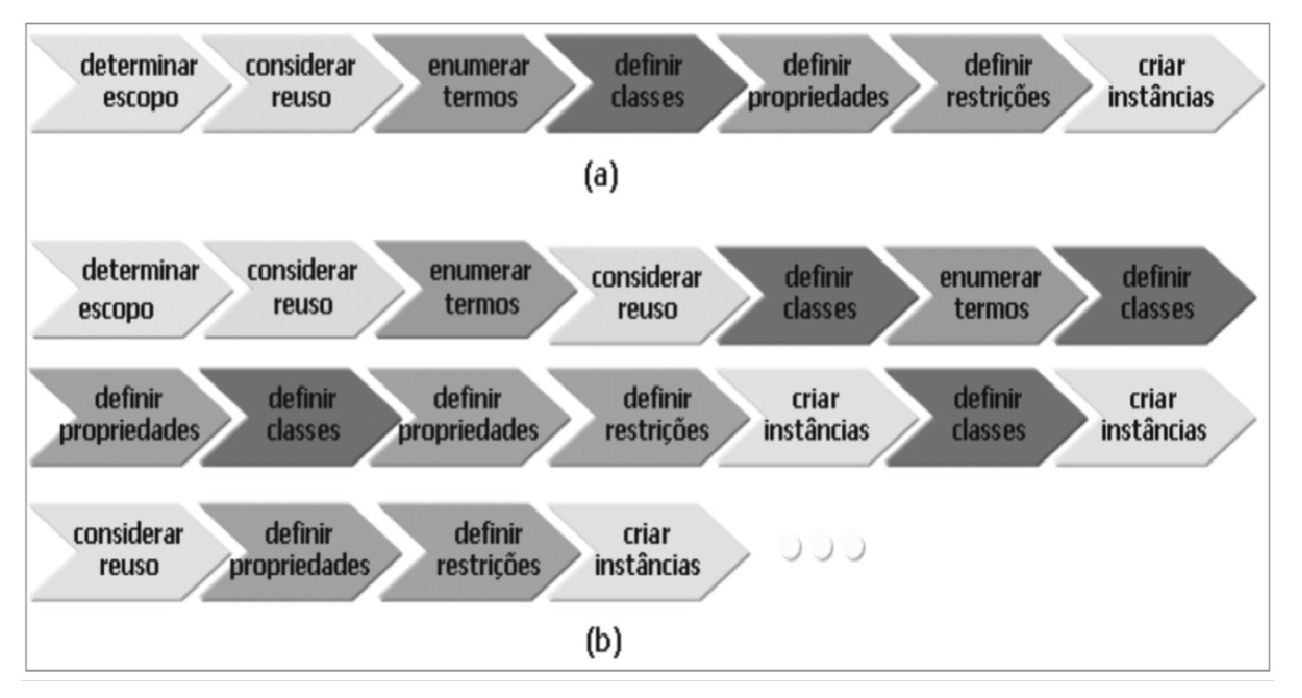
\includegraphics[keepaspectratio=true,scale=0.5]{figuras/ab.eps}
	\caption{Processo de desenvolvimento pelo guia Ontology Development 101}
	\label{fig:ab}
\end{figure}


Como podemos observar, a figura \ref{fig:ab} ilustra (a) os sete passos sugeridos pelos pesquisadores e (b) um exemplo de como estes passos podem ser empregados no processo de desenvolvimento de uma ontologia.
Este processo de projeto iterativo provavelmente continuará por todo o ciclo de vida da ontologia.

\begin{itemize}
 	\item \textbf{Passo 1}: Determinar o domínio e escopo da ontologia: o autor sugere começar o desenvolvimento da ontologia definindo seu domínio e escopo. Tais perguntas devem ser respondidas: “o que é o domínio que a ontologia irá cobrir?”, “para que tipos de perguntas a ontologia deve fornecer respostas?”, “quem vai usar e manter a ontologia?”. Acredita-se que as respostas para estas perguntas podem ajudar a limitar o escopo do modelo, mesmo que possivelmente sofra alterações durante o processo.
 	\item \textbf{Passo 2}: Considerar o reuso de ontologias existentes: nem sempre precisamos começar do zero, ainda mais se já existe algo ou parte de algo que queremos desenvolver. O autor sugere que sempre devemos considerar o reuso verificando se podemos aperfeiçoar e alargar as fontes existentes para nosso domínio particular e tarefa. Isto é ainda mais válido se queremos interagir com outras aplicações que já fazem uso de ontologias.
	\item \textbf{Passo 3}: Enumerar termos importantes da ontologia: o autor trás a utilidade deste passo sobre três âmbitos diferentes. O primeiro deles é para que exista uma lista de todos os termos que gostaríamos. Os outros dois são: para fazer declarações ou para explicar a um usuário. Este passo tende a responder as seguintes perguntas: “quais são os termos que gostaria de falar?”, “que propriedades que esses termos têm?” “o que nós gostamos de dizer sobre esses termos?”.
	\item \textbf{Passo 4}: Definir as classes e hierarquia de classes: dentre as várias abordagens possíveis para o desenvolvimento de uma hierarquia de classes, o autor fala mais especificamente sobre três, a saber: o processo de desenvolvimento top-down, o processo de desenvolvimento bottom-up e a combinação dos dois anteriores.
	\item \textbf{Passo 5}: Definir as propriedades da classe - slots: as classes por si só não fornecem informações suficientes para responder as questões de competência do passo 1. Uma vez definida as classes, faz-se necessário a descrição da estrutura interna de cada uma delas. Os slots, portanto, assemelham-se aos atributos de uma classe se compararmos ao conceito OO (orientado a objetos).
	\item \textbf{Passo 6}:Definir os facets dos slots: slots pode ter diferentes facets que descrevem o tipo de valor, os valores permitidos, o número dos valores (cardinalidade), e outras características dos valores que o slot pode tomar. Os facets assemelham-se ao tipo de dado um um atributo de classe pode assumir se compararmos ao conceito OO.
	\item \textbf{Passo 7}: Criar instâncias: o último passo é a criação de instâncias individuais de classes na hierarquia. Definindo uma instância individual de uma classe requer (1) a escolha de uma classe, (2) a criação de uma instância individual dessa classe, e (3) o preenchimento dos valores de slot. A instância, aqui no processo Ontology Development 101, possui a mesma definição da encontrada para uma instância no conceito OO. Portanto, finalmente são criadas as instâncias da ontologia a partir da definição das classes, valorando suas propriedades de dados e relações.
\end{itemize}

\subsection{On-to-knowledge}

Fruto da cooperação de várias entidades européias, esta metodologia foi desenvolvida para construção de ontologias para serem empregadas em Sistema de Gestão do Conhecimento \cite{STUDER}. A figura abaixo mostra as cinco fases definidas pela metodologia:

 \begin{figure}[ht]
	\centering
		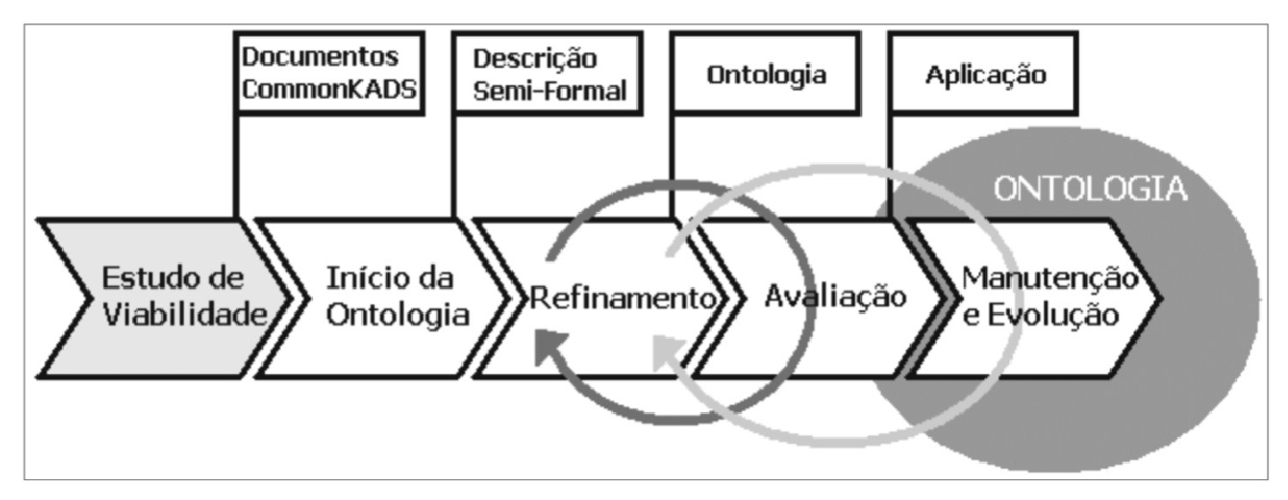
\includegraphics[keepaspectratio=true,scale=0.5]{figuras/on-to-kon.eps}
	\caption{Processo de desenvolvimento da metodologia On-to-Knowledge}
	\label{ontoko}
\end{figure}

O estudo de viabilidade é uma fase anterior ao desenvolvimento efetivo da ontologia, onde os problemas serão elicitados objetivando o mapeamento da real necessidade do desenvolvimento de uma ontologia.

Fazendo uma analogia ao processo de desenvolvimento de software, esta fazendo objetiva a criação de documentos de especificação de requisitos onde o domínio e os objetivos da ontologia serão definidos, são utilizados padrões de projeto, fontes de conhecimento são identificadas, atores e cenários são definidos, questões de competência são enumerados, o ambiente de desenvolvimento da ontologia é definido, entre outros.

Como dito anteriormente, esta metodologia foi elaborada para construção de ontologias voltada para o Sistema de Gestão e Conhecimento e é na fase de refinamento que isso realmente acontece partindo dos documentos produzidos nas fases anteriores. Para tanto, os engenheiros do conhecimento se valem de técnicas de elicitação do conhecimento ao interagir com os especialistas de domínio, modificando e estendendo a ontologia em desenvolvimento na direção de uma versão estável.

Já na fase de avaliação, o objetivo dela é a aferição da completude e precisão da ontologia mediante a documentação gerada durante o desenvolvimento da ontologia e um frame de referência, o qual pode corresponder às questões de competência enumeradas na fase “início da ontologia”. 

E, por último e não menos importante, temos a fase de manutenção e evolução cuja responsabilidade é da organização que utilizará a ontologia. É importante ter ciência dos atores responsáveis pela manutenção da ontologia e das regras para sua manutenção.

\subsection{Methontology}

Sendo a mais utilizada para construção de ontologias, a Methontology é uma metodologia de desenvolvimento de ontologias que foi fortemente influenciada pelas metodologias de Engenharia de Software e Engenharia do Conhecimento idealizada por um grupo que compõe o Laboratório de Inteligência Artificial e que trabalham com Engenharia de Ontologias da Universidade Politécnica de Madri, da Espanha,  em 1997 \cite{gomez}.

 \begin{figure}[ht]
	\centering
		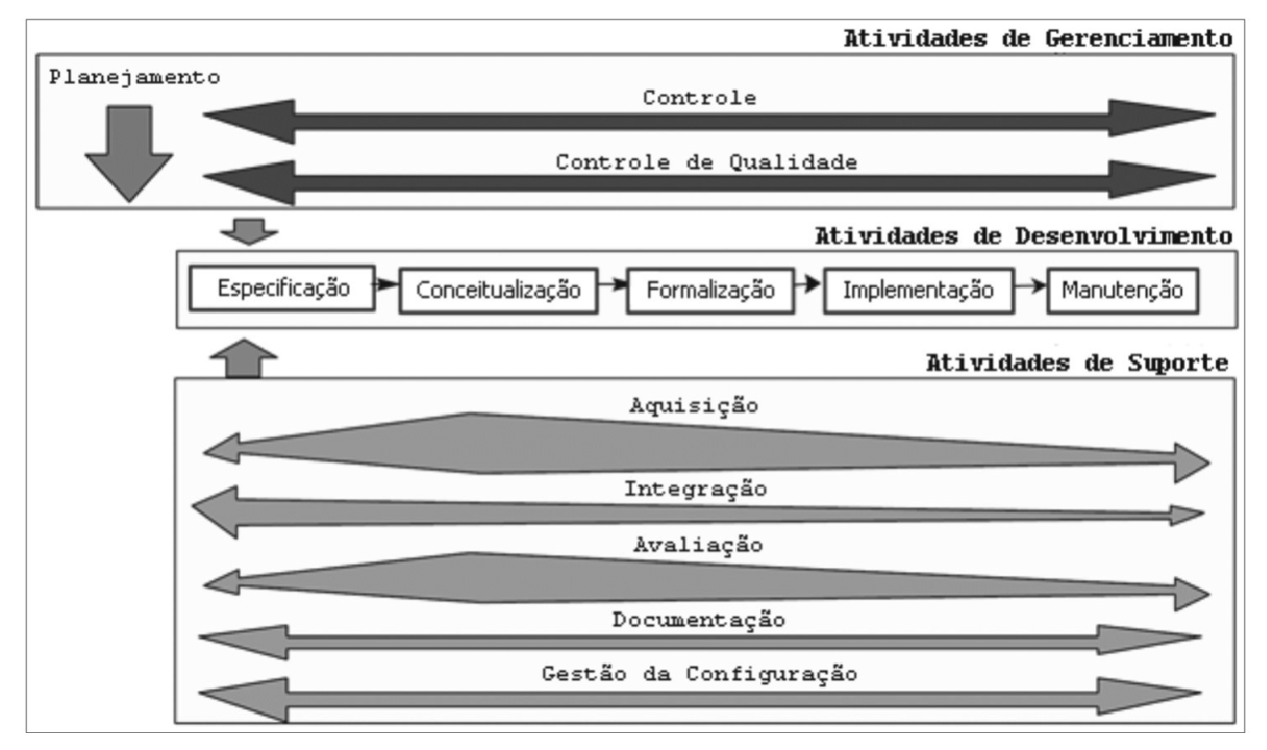
\includegraphics[keepaspectratio=true,scale=0.5]{figuras/metodology.eps}
	\caption{Processo de desenvolvimento da metodologia On-to-Knowledge}
	\label{metodology}
\end{figure}

A construção de ontologias segundo este método envolve estágios de: especificação, aquisição do conhecimento, conceitualização, formalização, integração, implementação, avaliação, documentação e manutenção. A partir destes estágios o conhecimento é representado nas ontologias.	

A Methontology possibilita a construção de ontologias no nível do conhecimento, sendo caracterizada por apresentar: uma identificação do processo de desenvolvimento de ontologias; um ciclo de vida baseado em evolução de protótipos; e técnicas particulares para alcançar cada uma de suas atividades [5]. Esta metodologia propõe um ciclo de vida baseado na evolução de protótipos para o desenvolvimento de ontologias porque permite adicionar, mudar ou remover termos em cada nova versão, ou seja, novo protótipo da ontologia.

Tem-se como característica também deste método, a sua forma estruturada para a construção de ontologias, que é composta por alguns estágios descritos a seguir \cite{mariano}:

\begin{itemize}
\item especificação: objetiva a elaboração de um documento, utilizando-se linguagem natural, contendo informações como: o principal objetivo da ontologia e seus demais propósitos;
\item aquisição de conhecimento: busca as possíveis fontes de conhecimentos, tais como entrevistas com especialistas do domínio, consulta a livros, ontologias já existentes, entre outros. Apesar de ser um estágio inicial, deve estar presente em todos os outros;
\item conceitualização: considerada como a principal fase desta metodologia. Trata da estruturação do domínio do conhecimento, em um modelo conceitual. Baseia-se no vocabulário adquirido com as fases anteriores, objetivando a descrição dos problemas enfrentados e as suas possíveis soluções;
\item formalização: o modelo conceitual criado no estágio anterior é transformado em um modelo formal, ou seja, é representado por meio de uma linguagem formal;
\item integração: objetiva a integração da ontologia que se está construindo as outras já existentes. Envolvendo assim, a busca por ontologias que melhor se adequem a conceitualização utilizada;
\item implementação: o modelo conceitual gerado é implementado de forma a ser computável;
\item avaliação: trata da avaliação em si da ontologia e deve considerar os processos de verificação e validação;
\item documentação: auxilia na possível manutenção, e facilita uma de suas vantagens, a reutilização. Compõe-se por alguns elementos, como documentos de: especificação dos requisitos, alcançados após a especificação da ontologia; aquisição de conhecimento; modelo conceitual, obtido após a conceitualização; formalização e avaliação;
\item manutenção: constituem as alterações quando necessárias, para possíveis melhorias ou correções.
\end{itemize}

\subsection{Construção da Ontologia}

Para  o desenvolvimento da ontologia, os autores sugerem um processo para a construção, nomeado de Ontology Development 101. Este processo é composto por uma série de passos iterativos, livremente executados na construção da ontologia.\cite{MCGUINNESS}

A figura \ref{fig:ab} ilustra os sete passos sugeridos - pelos pesquisadores - para a construção da ontologia.

Uma vez que as atividades são executadas de forma livre, a figura \ref{fig:ab} mostra um exemplo de como as atividades podem ser empregadas no decorrer do desenvolvimento da ontologia.

De forma geral, a atividade de determinar escopo da ontologia deve-se identificar claramente o propósito e os cenários de utilização da ontologia a ser desenvolvida. “O que abrange o domínio da ontologia?”, “para que se utilizará a ontologia?”, “que questões a ontologia deveria responder?”, “quem utilizará e manterá a ontologia?” são exemplos de questões que norteiam a determinação do domínio e escopo no desenvolvimento de uma ontologia.

Considerar o reuso de ontologias existentes: é aconselhável verificar a existência de ontologias que podem ser reutilizadas em um novo projeto de ontologia, a fim de não se “reinventar a roda” ou proporcionar a interação da ontologia desenvolvida com outras aplicações.

Enumerar termos importantes do domínio da ontologia: relacionar uma lista de termos presentes no discurso do domínio da ontologia. A relação de termos é importante para os passos subsequentes do guia, como definir classes, definir propriedades e definir instâncias.

Definir as classes do domínio e a hierarquia de classes: a partir da lista de termos, extraem-se aqueles que descrevem objetos, os quais genericamente representam classes. Com um conjunto de classes definido, deve-se organizar as classes de forma hierárquica, considerando um nível de abstração mais geral em direção as classes específicas.

Definir as propriedades das classes: a partir da lista remanescente de termos, deve ser observados se eles correspondem a propriedades de dados ou de relações de classe para uma determinada classe.

Definir as restrições das propriedades: caso uma propriedade de classe seja de dados, observa-se o tipo de dado que a propriedade comporta (strings ou número, por exemplo). Caso a propriedade seja uma relação, deve-se definir a que classes a relação aponta. Restrições sobre cardinalidade e valores válidos para as propriedades também devem ser considerados neste passo.

Criar as instâncias do domínio: finalmente, criam-se as instâncias da ontologia a partir da definição das classes, valorando suas propriedades de dados e relações.

\chapter{Cronograma}\label{cap4}

Para a construção de qualquer ferramenta computacional, é essencial a definição e a execução do cronograma. Uma vez que o objetivo desse artigo é um plano para o desenvolvimento de uma ontologia, a seguir será apresentado um cronograma que servirá como guia para o cronograma da equipe de desenvolvimento da ontologia de audiobooks, , sendo idealizada com base nas metodologias descritas neste artigo, na secção 3 deste relatorio.

 \begin{figure}[ht]
  \centering
    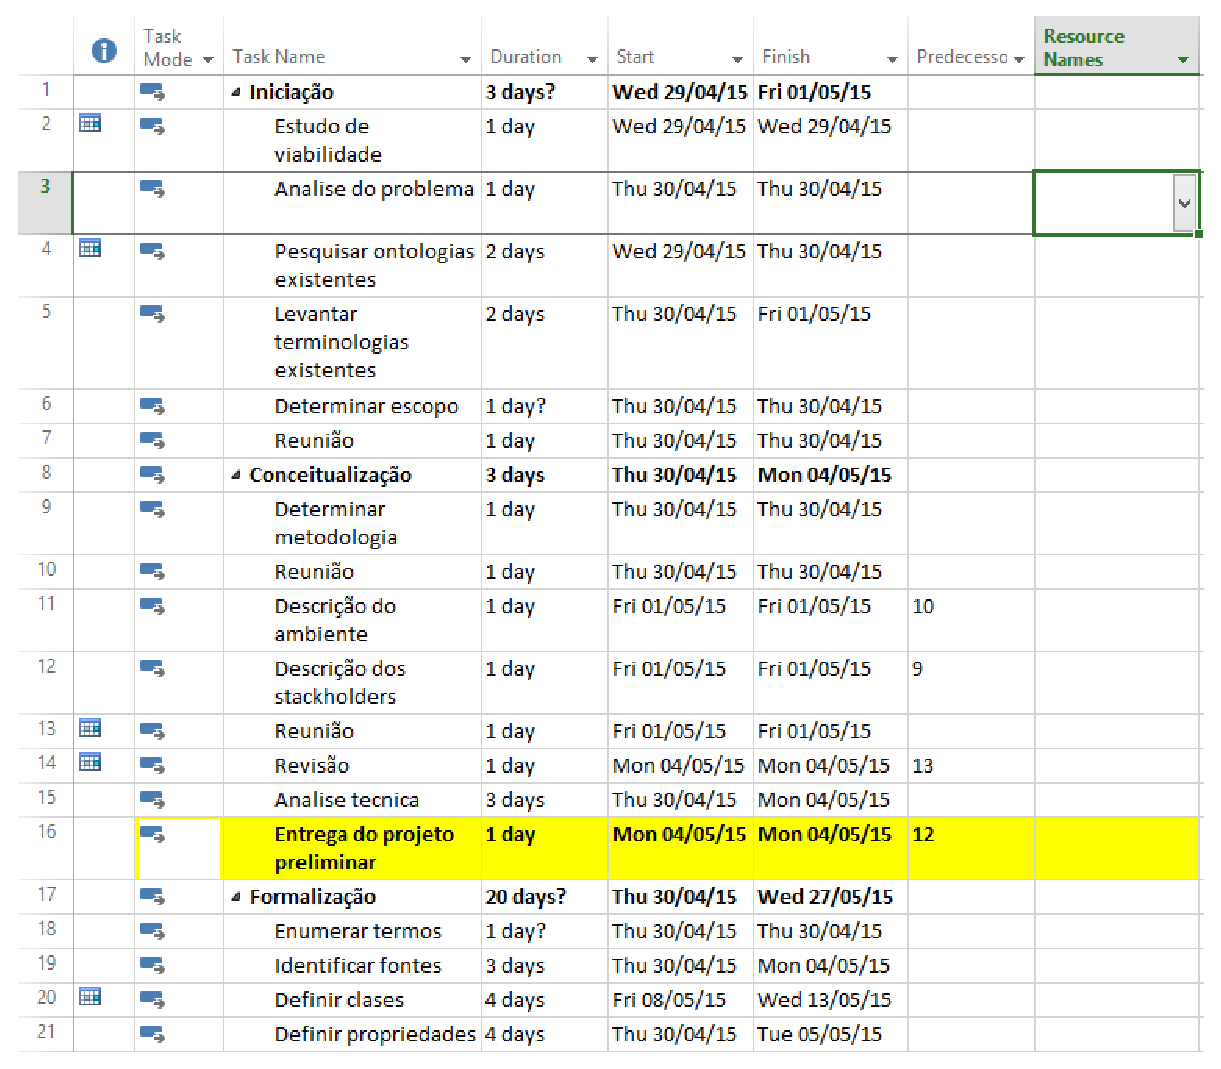
\includegraphics[keepaspectratio=true,scale=0.5]{figuras/cronograma1.eps}
  \caption{Cronograma do projeto}
\end{figure}

 \begin{figure}[ht]
  \centering
    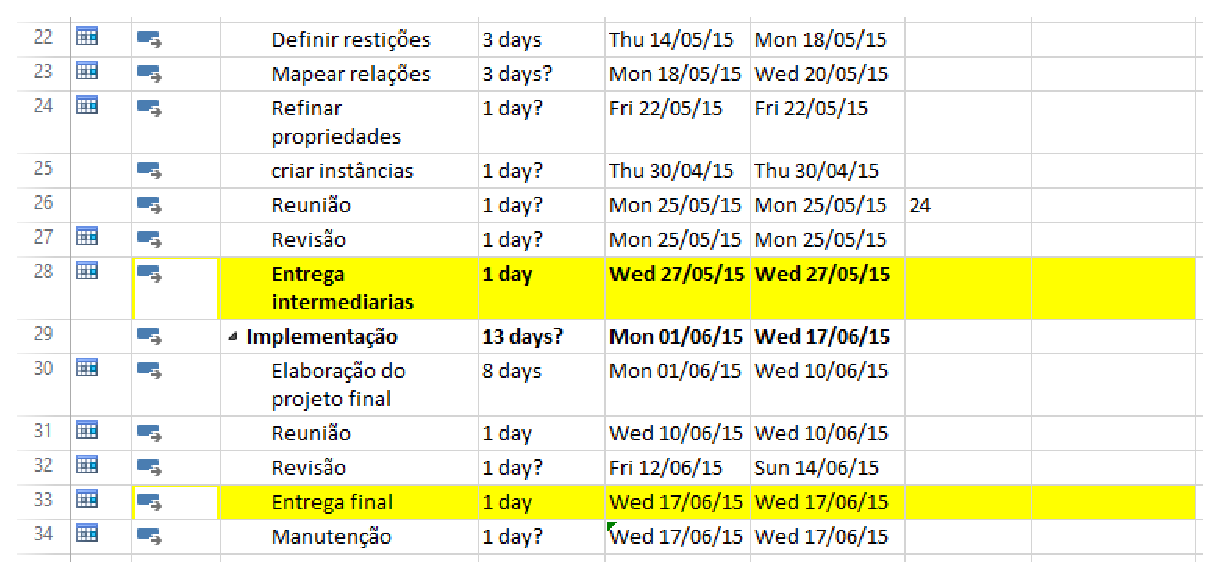
\includegraphics[keepaspectratio=true,scale=0.5]{figuras/cronograma.eps}
  \caption{Cronograma do projeto - continuação}
\end{figure}

\section{Processo e Atividades}

Os processos e atividades levantas aqui são baseadas no cronograma da sessão anterior.

 \begin{figure}[H]
  \centering
    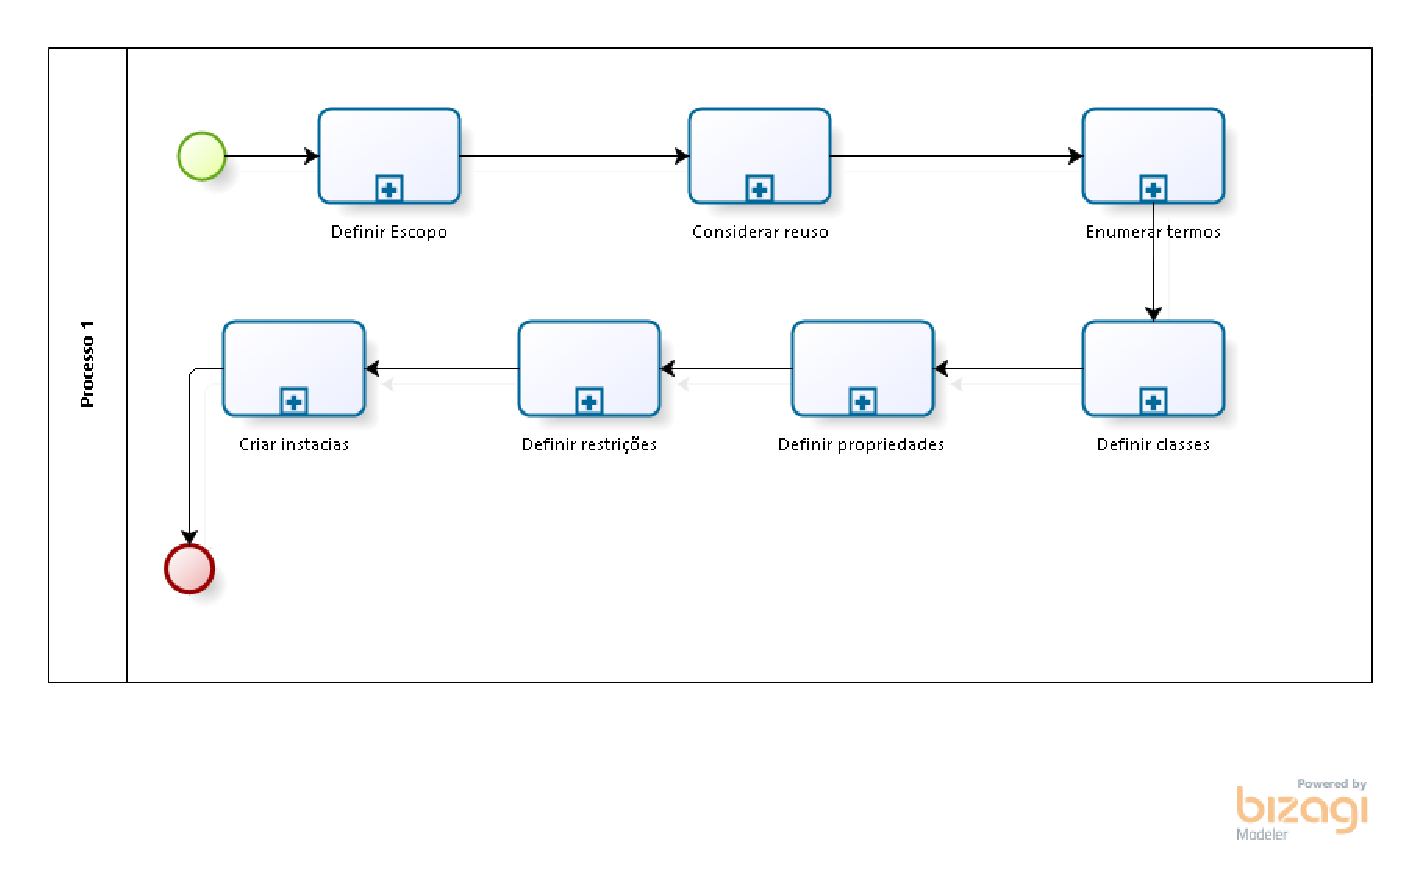
\includegraphics[keepaspectratio=true,scale=0.5]{figuras/Geral.eps}
  \caption{Processo Geral}
\end{figure}

 \begin{figure}[H]
  \centering
    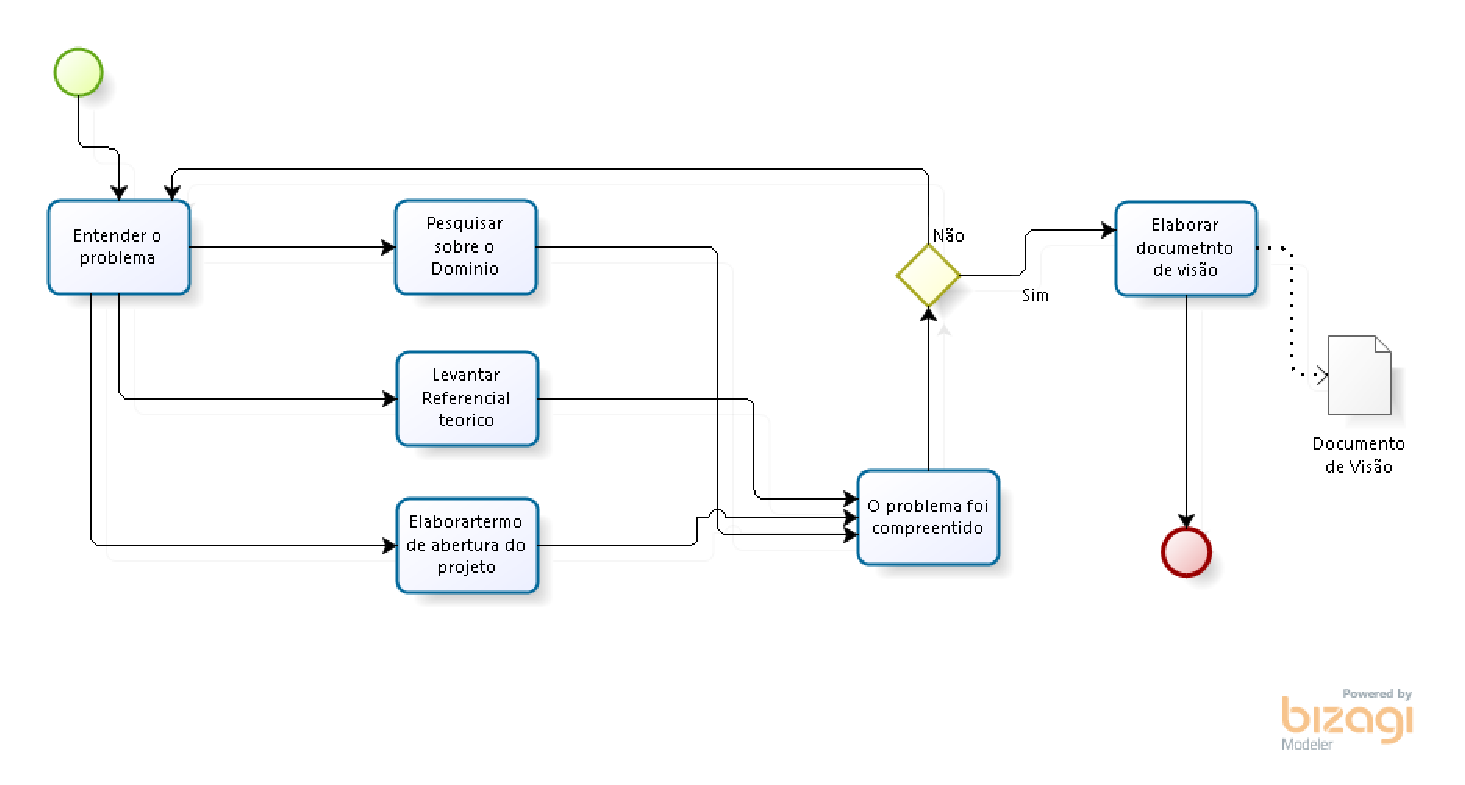
\includegraphics[keepaspectratio=true,scale=0.5]{figuras/Definir_escopo.eps}
  \caption{Atividade Definir escopo}
\end{figure}

 \begin{figure}[H]
  \centering
    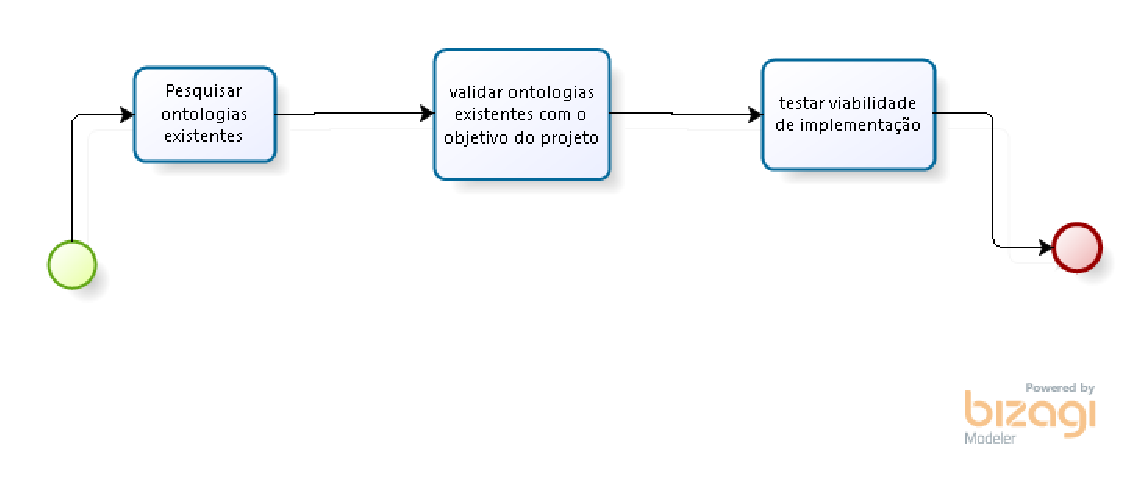
\includegraphics[keepaspectratio=true,scale=0.5]{figuras/Considerar_reuso.eps}
  \caption{Atividade considerar reuso}
\end{figure}

\begin{figure}[H]
  \centering
    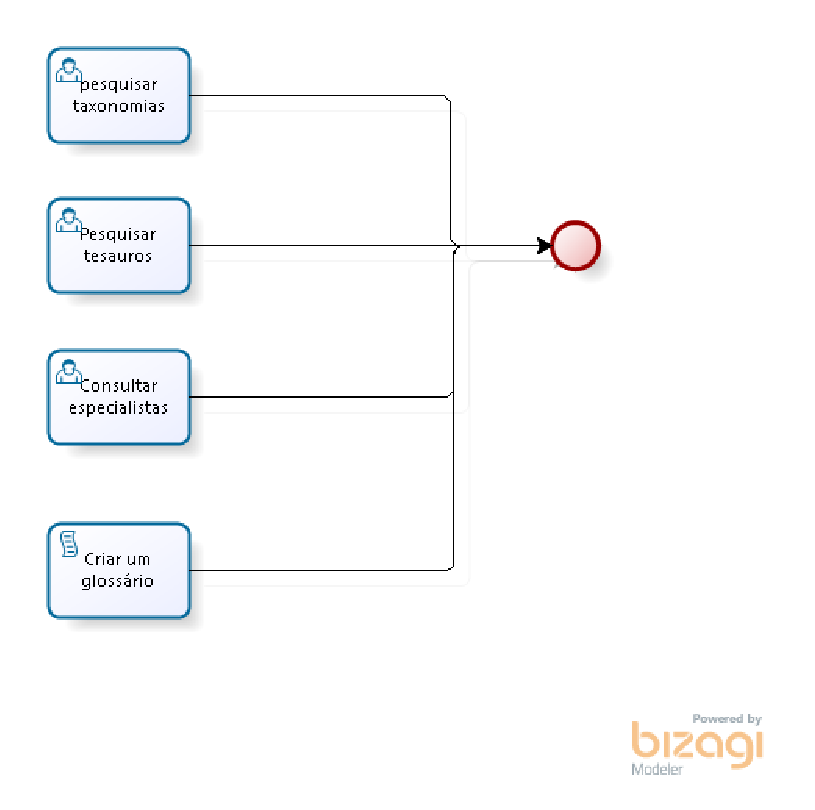
\includegraphics[keepaspectratio=true,scale=0.5]{figuras/Enumerar_termos.eps}
  \caption{Atividade enumerar termos}
\end{figure}

 \begin{figure}[H]
  \centering
    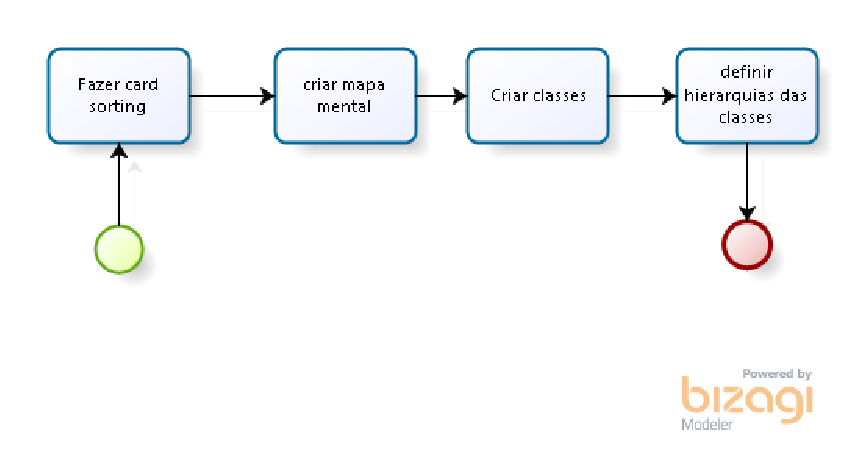
\includegraphics[keepaspectratio=true,scale=0.5]{figuras/Definir_classes.eps}
  \caption{Atividade definir classes}
\end{figure}

\begin{figure}[H]
  \centering
    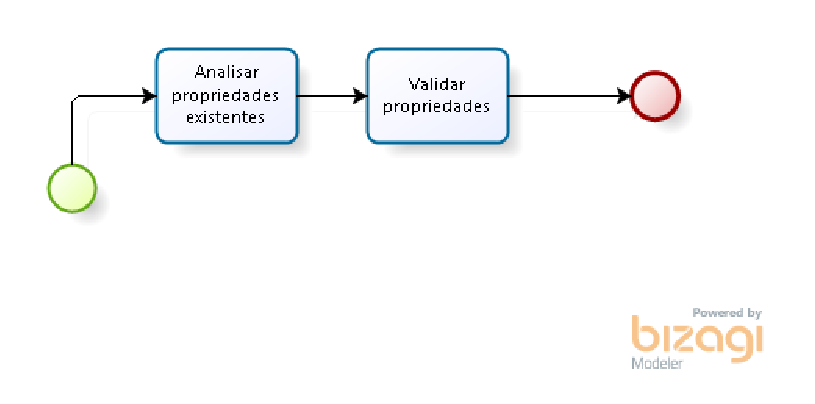
\includegraphics[keepaspectratio=true,scale=0.5]{figuras/Definir_propriedades.eps}
  \caption{Atividade definir propriedades}
\end{figure}

\begin{figure}[H]
  \centering
    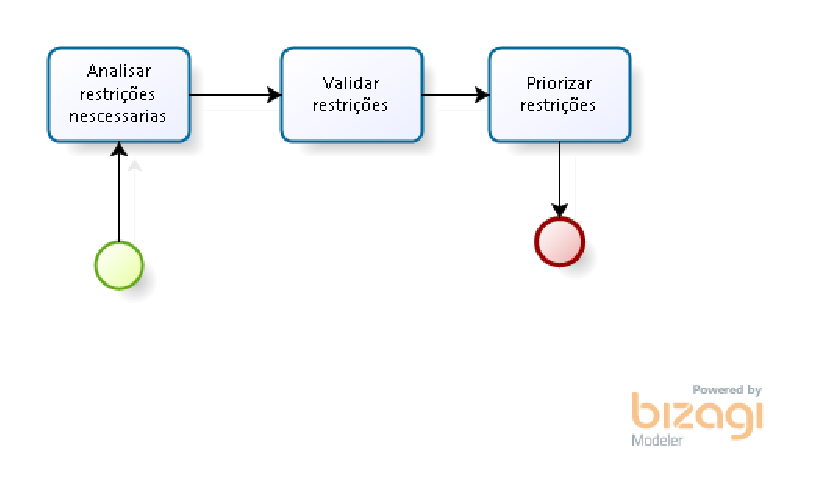
\includegraphics[keepaspectratio=true,scale=0.5]{figuras/Definir_restricoes.eps}
  \caption{Atividade definir restrições}
\end{figure}

\begin{figure}[H]
  \centering
    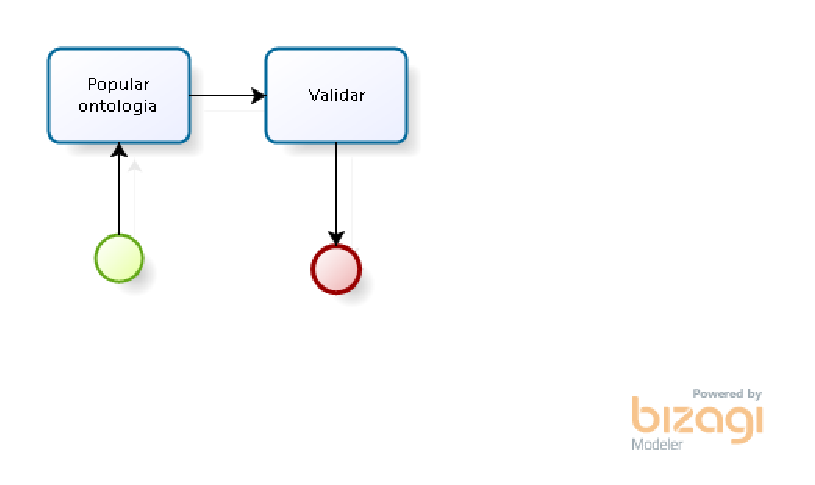
\includegraphics[keepaspectratio=true,scale=0.5]{figuras/Criar_instancias.eps}
  \caption{Atividade criar instancias}
\end{figure}

\section{Esforço realizado para a construção da ontolgoia}

Nessa sessão, será abordado a uma pespectiva da equipe necessária para a construção da ontologia de audiobooks, assim como o custo e horas de trabalho.

\subsection{Equipe}

O gerenciamento do time do projeto é essencial para que o mesmo seja concluído com êxito, no prazo acordado, de acordo com o escopo solicitado e com o custo inicialmente planejado. O gerente de projeto conduzirá o desenvolvimento das habilidades e conhecimentos dos membros da equipe no dia a dia do projeto buscando tornar essa, uma equipe de alto desempenho. \cite{CHIAVENATO}

Para o desenvolvimento do projeto proposto por esse trabalho, é recomendado um equipe de três membros. Sendo eles: um especialista em audiobooks, um \textit{expect} na ferramenta de desenvolvimento de ontologias protegê, e um especialista em \textit{mind map}.

O três especialistas trabalharam em conjunto, cada um contribuindo com o seu conhecimento, para a abstração e implementação da ontologia no mundo de audibooks.
O especialista em audibooks, trabalhará mais fundo na parte da abstração de todas as informações que descrevem uma biblioteca de audiobooks. 
Já o especialista em mind map, poderá contribuir na estruturação da abstração criada em um forma eficiênte e em seguida o especialista em protegê implementará as abstrações/mind map na ferramenta, criando assim a ontologoia.

\subsection{Horas e Custo}

O cálculo do custo da ontologia, será baseado na forma de cálculo de custo que um software normal, ou seja, horas de trabalho x custo por hóra.

Pela experiência que os autores tiveram na duração da disciplina de Web Semântica, as horas gastas para a criação de uma ontologia são por área:

\begin{itemize}
	\item Especialista em audiobooks: 9 horas
	\item Especialista em mind map: 11 horas
	\item Especialista em ontologia: 25 horas
\end{itemize}

Preço estimado da hora de cada especialista: 

\begin{itemize}
	\item Especialista em audiobooks: uma vez que audiobooks são basicamente livros em forma de áudios, esse membro pode ser um bibliotecário que ganha em média 47 reais a hora. \cite{bibliotecaria}
	\item Especialista em mind map: o papel desse integrate pode ser desempenhado por um análista de banco de dados que ganha em média 33 reais a hora.\cite{profissionaisti}
	\item Especialista em ontologia: esse papel pode ser desenpenhado por um engenheiro de software que ganha em média 40 reais a hora. \cite{profissionaisti}
\end{itemize}

Dessa forma um valor estimado da ontologia é definido na conta a seguir.

\begin{equation}
Valor = (9 * 47) + (11 * 33) + (25 * 40) = 1786 reais
\end{equation} 




